\documentclass[journal, 11pt]{IEEEtran}

\usepackage{epsfig,rotating,setspace,latexsym,amsmath,epsf,amssymb,bm,amsbsy}
\usepackage{cite,graphicx,color,subfigure,here}
\usepackage{amsmath}
\usepackage[normalem]{ulem} 
\usepackage{algorithm}
\usepackage[noend]{algpseudocode}
\usepackage{epstopdf}
\usepackage{scrextend}
\usepackage{ifpdf}
\usepackage{authblk}
\usepackage{caption2}
\usepackage{caption3}
\usepackage[english]{babel}
\usepackage{dsfont}

\newcommand{\ba}{\begin{align}}
\newcommand{\ea}{\end{align}}


\begin{document}
\title{Cognition in Connected Vehicles}

\author{Bengi Aygun$^\dag$, Mahni Shayganfar$^*$, and Alexander M. Wyglinski$^\dag$\\
\normalsize $^\dag$Department of Electrical and Computer Engineering, Worcester Polytechnic Institute, Worcester, MA\\
\normalsize $^*$Department of Computer Science, Worcester Polytechnic Institute, Worcester, MA\\
\normalsize Email: \{baygun, alexw\}@wpi.edu, mshayganfar@wpi.edu}

\maketitle

\begin{abstract}
In this paper,
\end{abstract}

\begin{keywords}
cognition, connected vehicles ...
\end{keywords}%

\IEEEpeerreviewmaketitle
\section{Introduction}
%
Intelligent transportation systems (ITS) will form an integral part of society's
transportation infrastructure within few years

\subsection{Roads as Social Environments}

A social environment refers to an individual's physical surroundings, resources
and social relationships. A social relationship includes the interaction between
two or more individuals in the environment. A social relationship is the most
dynamic part of a social environment. Hence, developing and maintaining positive
social relationships is crucial for a social environment and is influenced by
the individuals' quality of interaction. Roads are social environments in which
individual vehicles interact with each other through their ``nonverbal"
behaviors obeying the same traffic law. However, there are many violations of
the laws on the roads all over the world in daily basis which consequently leads
to expensive and sorrowful failures. What causes these failures is mostly the
failure of the drivers to effectively interpret their driving environment and
make an appropriate decision with respect to their constraints such as lack of
time, lack of perception, and plethora of cognitive load. Therefore, it is
crucial to involve awareness in the vehicles to share the meaning of what they
dynamically perceive rather than broadcasting the data coming from their sensory
system. For example, any sensory information leading to an alert on a particular
vehicle does not necessarily have the same meaning both for the occupants and
the neighbors of that vehicle. The alert warns the occupants of the vehicle to
be aware of an internal failure (e.g., malfunction in the transmission system),
or an external adversary (e.g., an unexpected leaping of an animal into the
road). The same alert has a different meaning for the close vehicle approaching
from behind; no matter what caused the alert in the leading vehicle, the
posterior vehicle should slow down effective immidiately. However, the same
alert can be interpreted in a totally different way for a neighbor in front of
the originally alerted vehicle. In fact, this vehicle can ignore the received
alert and continue the safe drive. Ultimately, these type of improvements leads
to a higher quality of vehicles' interaction which consequently increases the
safety of the roads.

% \subsection{Driving Needs Pareto Optimal Decisions}

\subsection{Cognition Systems}

Integration of cogniton into connected vehicles needs us to understand the
building blocks of cognition, how do they relate to each other, and what
functional operations they provide. We choose Newell's general theory of
cognitive control, PEACTIDM \cite{newell:unified-cognition}, to describle the
underlying abstract processes of a cognitive system. PEACTIDM is a theory of
cognitive control where cognition is decomposed into a set of eight abstract
functional operations \cite{newell:unified-cognition} all of which are
hypothesized as the building blocks of one's immediate behavior. Figure
\ref{fig:peactidm} shows the sequence of PEACTIDM's building blocks.

\textit{Perceive} is the reception of raw sensory data. For instance, connected
vehicles receive data from both their own local sensory system (e.g., GPS) and
their neighbor vehicles (e.g., an abrupt change in their velocities).
\textit{Encode} is the transformation of the sensory data into features that the
cognitive system can process. In the cognitive architectures using BDI paradigm
each sensory data will be tranformed into a new \textit{belief}. The cognitive
architecture will be able to use these beliefs in different processes. For
example, in connected vehicles there will be a belief about the current
accelaration value of the vehicle which corresponds to the sensory data
indicating this value. \textit{Attend} is the act of shifting or maintaining the
focus of attention on an event. For instance, an alert raised because of a
sudden speed reduction of multiple leading neighbor vehicles needs to be
attended immediately while the same alert does not need the same level of
attention if the leading vehicles are a few miles apart. \textit{Comprehend} is
the act of trnasforming an event into a goal or task-spcific representation and
inferring the curent status of the world. For instance, a vehicle receiving an
alert requiring an immediate reaction needs to identify the cause of the problem
even though the alert has raised and received from another vehicle. Thus, the
receiver of the alert can apply replanning if necessary.

\textit{Tasking}

\begin{figure}[tbh]
  \centering
  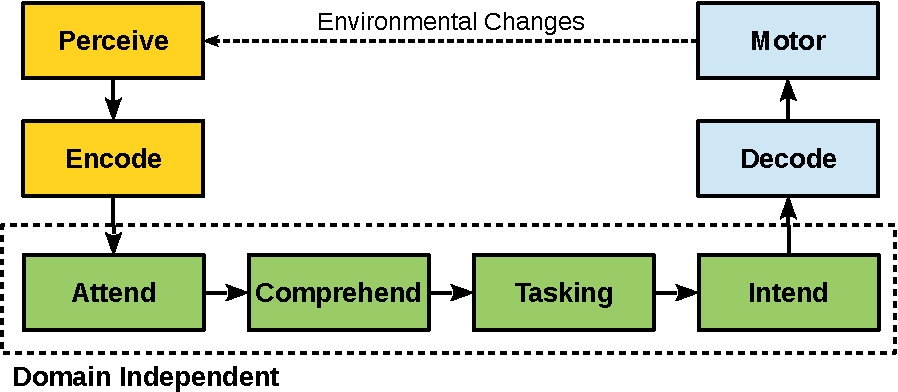
\includegraphics[width=0.485\textwidth]{figs/peactidm-croped.pdf}
  \caption{{\fontsize{10}{10}\selectfont PEACTIDM}}
  \label{fig:peactidm}
\end{figure}

\section{{\fontsize{11.5}{9}\selectfont Affective Motivational Collaboration
Theory}}
\label{sec:amct}

\textit{Affective Motivational Collaboration Theory} is about the interpretation
and prediction of observable behaviors in a dyadic collaborative interaction.
This theory is built on the foundations of the \textit{SharedPlans} theory of
collaboration \cite{grosz:plans-discourse} and the \textit{cognitive appraisal}
theory of emotions \cite{gratch:domain-independent}. The theory focuses on the
processes regulated by emotional states. The observable behaviors represent the
outcome of reactive and deliberative processes related to the interpretation of
the self's relationship to the collaborative environment. Affective Motivational
Collaboration Theory aims to explain both rapid emotional reactions to events as
well as slower, more deliberative responses. The reactive and deliberative
processes are triggered by two types of events: \textit{external} events, such
as the other's \textit{utterances} and \textit{primitive actions}, and
\textit{internal} events, comprising changes in the self's mental states, such
as belief formation and emotional changes. Affective Motivational Collaboration
Theory explains how emotions regulate the underlying processes when these events
occur during collaboration. This theory elucidates the role of motives as
goal-driven affect-regulated constructs with which an agent can form new
intentions to cope with internal and external events. The focus of underlying
mechanisms is on the ones depicted as mental processes in Figure
\ref{fig:cpm} along with the mental states.

\begin{figure}[tbh]
  \centering
  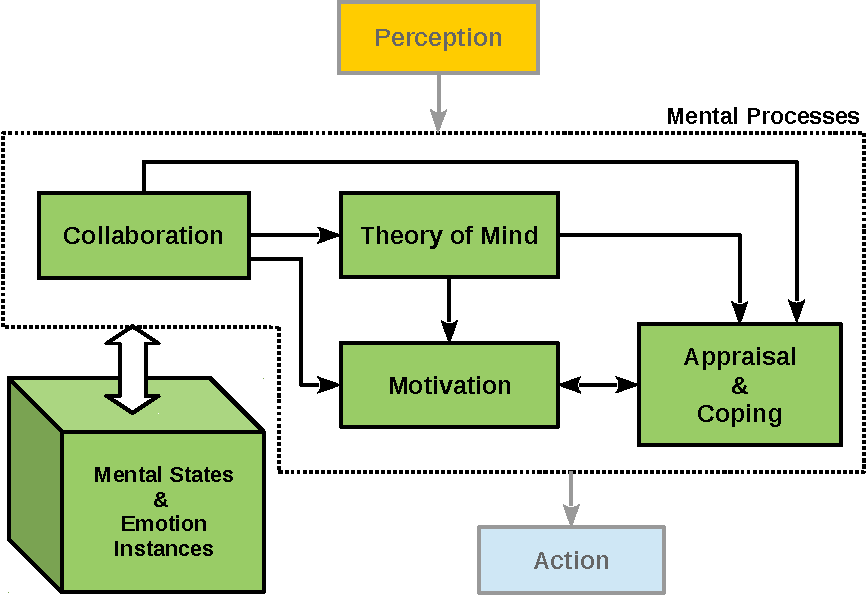
\includegraphics[width=0.485\textwidth]{figs/theory-general-croped.pdf}
  \caption{{\fontsize{10}{10}\selectfont Computational framework based on
  Affective Motivational Collaboration Theory (arrows indicate primary
  influences between mechanisms).}}
  \label{fig:cpm}
\end{figure}

The \textit{Mental States} includes self's (robot's) beliefs, intentions,
motives, goals and emotion instances as well as the anticipated Mental States of
the other (human). The \textit{Collaboration} mechanism maintains constraints on
actions, including task states and the ordering of tasks. The
\textit{Collaboration} mechanism also provides processes to update and monitor
the shared plan. The \textit{Appraisal} mechanism is responsible for evaluating
changes in the self's Mental States, the anticipated Mental States of the other,
and the state of the collaboration environment. The \textit{Coping} mechanism
provides the self with different coping strategies associated with changes in
the self's mental states with respect to the state of the collaboration. The
\textit{Motivation} mechanism operates whenever the self a) requires a new
motive to overcome an internal impasse in an ongoing task, or b) wants to
provide an external motive to the other when the other faces a problem in a
task. The \textit{Theory of Mind} mechanism is the mechanism that infers a model
of the other's anticipated mental state. The self progressively updates this
model during the collaboration.

\section{Proposed Cognition Mechanism in Connected Vehicles}
\label{sec:cogInCv}
%

%
%
%
%%%%%%%%%%%
%
%
%
%
\section{Case Study}
\label{sec:caseStudy}
%
%
\section{Future Works}
\label{sec:futureWorks}
%
%
%
%\begin{figure}[!h]
%\centerline{\epsfig{figure =figs/PerrorSurface.eps, height=1.8 in}}
%\caption{Probability of incorrect detection by changing SNR and detection threshold. For each SNR value, there is only one minimum point since the the function is convex.}\label{PerrorSurface} 
%\end{figure}
%


\section{Conclusion}
\label{Conc}
%

\bibliographystyle{IEEEtran}
\bibliography{mshayganfar}
% \bibliography{referencesVTM}
\end{document}
